
\chapter{Implementace rozšíření simulátoru}
\label{Implementacerozs}
% Java

Tato kapitola se zaměřuje na konkrétní postup implementace úprav a rozšíření simulátoru, které byly popsány v sekci \ref{rozsireniJava}.
Podrobněji bude popsána hlavní simulační smyčka, zpracování assembleru a implementace serverového rozhraní.

\section{Refaktorizace}
% cache, registry, volání bloků, prediktory, labels
% přehled změn popsaných v této kapitole

Refaktorizace kódu byla prvním implementačním úkolem.
Probíhala zároveň s~analýzou a návrhem a sloužila jako příprava k~pozdějšímu přidávání nových funkcí.
Úpravy v~této fázi byly menšího rozsahu, především se jednalo o~lokální změny v~rámci funkcí a přidávání komentářů.
V~druhé fázi přišly na řadu větší celky, včetně jejich rozhraní.
Důvodem k~zásahu bylo buď zvýšení čitelnosti, nové požadavky na modul, nebo potřeba změnit reprezentaci pro snadnou serializaci (a následné zobrazení na webu).

Určit hranici mezi refaktorováním a novou implementací není jednoduché.
Většina modulů se změnila zásadním způsobem, včetně způsobu interakce mezi moduly.
Příloha \ref{prevzanaPrace} uvádí tabulku s~přehledem jednotlivých modulů aplikace a můj přínos.

% SimCodeModel - zrušena dědičnost, exceptions, sloučení se stavem ROB (předělání renamedLine)
Třída \texttt{SimCodeModel} představující instrukci v~systému obsáhla stavové informace z~ROB, nově také nese informace o~vyvolané výjimce a lépe strukturované informace o~skoku a své pozici v~kódu.

% Load/Store - transakce
% TODO jak vypadala hlavní paměť dřív?
Paměťový modul (hlavní paměť a cache) zaznamenal významné změny, ale princip fungování zůstal stejný.
Tyto bloky nyní pracují v~\emph{transakčním režimu}.
Funkční bloky, které požadují data z~paměti generují nový objekt představující transakci.
Při registraci správa paměti tento objekt vyplní údajem o~délce vybavení transakce.
Transakce umožňují lehkou konfiguraci doby vybavení z~paměti, jsou kompatibilní s~vypláchnutím linky a obsahují metadata, která jsou zajímavá při interaktivní simulaci.

Není možné zmínit každé vylepšení.
Jako příklad menších úprav uvedu změnu vyjádření prediktorů skoků.
Původní návrh využíval dědičnosti tříd.
Implementace byla zredukována na jedinou třídu \texttt{BitPredictor}, kterou je možné parametrizovat.
Výsledkem bylo zjednodušení kódu (4 původní třídy byly sloučeny do jedné univerzální) a lepší kompatibilita se serializací do JSONu.

\subsection{Registry}
% Reference a lineární prohledávání registrového pole podle stringového jména
% Ukládání hodnoty jako double
% Držení stavu registru v jiné struktuře

Problémem jak z~výkonnostního tak z~návrhového hlediska byla práce s~registry.
Instrukce držely reference na registry jako řetězce s~jejich názvy (např. \texttt{\uv{x5}}, \texttt{\uv{tg24}}).
Při \emph{každém} přístupu k~hodnotě registru bylo nutné provést lineární vyhledávání nad celým registrovým polem, tedy nad stovkami registrů a pro každý prvek muselo proběhnout porovnání s~hledaným řetězcem.
Metadata registru byla navíc udržována v~jiné datové struktuře, takže bylo nutné provést druhé vyhledání.
Také bylo nutné tyto struktury udržovat synchronizované.

Reference v~podobě řetězců jsem nahradil opravdovými \emph{referencemi} na objekt.
Nyní přístup k~registru odpovídá následování ukazatele, což je mnohem efektivnější operace.
Registr je vyhledáván pouze jednou při inicializaci programu a jednou při přejmenování instrukce.

Nový návrh objektu \texttt{RegisterModel} obsahuje svůj datový typ a stav alokace.
Hodnota již není reprezentována datovým typem \texttt{double}, ale novým objektem třídy \texttt{Register\-Data\-Container}, která dokáže reprezentovat jak celá čísla, tak i čísla ve formátu plovoucí desetinné čárky.
Objekt zapouzdřuje pole 64 bitů v~podobě proměnné typu \texttt{long}, ke kterému nabízí jak přímý přístup, tak interpretovaný přístup.

Registr také obsahuje všechny informace nutné k~přejmenování.
Všechny registry mají počet referencí, architekturní registry využívají seznam přejmenování a spekulativní registry obsahují odkaz na odpovídající architekturní registr.

Díky detailním metadatům je možné registry v~interaktivní simulaci detailně zkoumat.

Další souvislostí je, že díky odkazovatelnosti na objekty \texttt{RegisterDataContainer} nemusí být hodnoty kopírovány mezi buffery (například v~blocích \texttt{issue} a \texttt{load buffer}). 

\section{Simulace}
\label{implSimulace}

Významnou změnou je nový způsob zpětné simulace navržené v~sekci \ref{backSimNewDesign}.
Bloky nyní neobsahují logiku pro zpětnou simulaci ani datové struktury, které byly pro zpětný chod nutné.
Kód se stal významně jednodušším, protože operace nyní nemusí být reverzibilní.

Původní implementace simulační logiky používala návrhové vzory jako \emph{Singleton} a \emph{Dependency Injection}, které komplikovaly vytváření instancí procesoru.
V~aplikaci navíc nemohlo souběžně existovat více instancí procesoru, což znemožnilo implementaci obsluhy dotazů na server.
Tento přístup také komplikoval testování procesoru jako celku.

Zapouzdřil jsem proto všechny bloky procesoru a jejich inicializaci do třídy \texttt{Cpu}.
Rozhraní pro vykonání simulace se stalo významně jednodušším.
Příklad provedení simulace je uveden v~kódu \ref{cpuApi}.
Po volání \texttt{execute} je objekt \texttt{cpu} ve stavu na konci simulace.
Tento stav je možné zkoumat v~rámci testu, nebo prezentovat uživateli.

\begin{lstlisting}[caption={Příklad spuštění simulace s~výchozí konfigurací a vlastním kódem.},captionpos=b,label=cpuApi]
SimulationConfig config = SimulationConfig.getDefaultConfiguration();
config.code = "addi x8, x8, 5";
Cpu cpu = new Cpu(config);
cpu.execute(false);
\end{lstlisting}

%step
Funkce \texttt{execute} je funkcí pro pohodlí při testování.
Pro potřeby interaktivní simulace existuje metoda \texttt{simulateState(targetTick)}, která ve smyčce volá \texttt{step}.
Detailnější popis rozhraní třídy Cpu je uveden v~sekci \ref{simLoop}.

% determinismus
Simulace je deterministická.
Determinismus je v~místech, kde se pracuje s~náhodou, docílen inicializací pseudonáhodného generátoru do stejného výchozího stavu.

\subsection{Inicializace a Hlavní smyčka simulace}
\label{simLoop}
% Vstupní bod, konfigurace, class Cpu init, zásobník (i zastavení simulace)
% step(), simEnded()
% Komunikace bloků, jejich pořadí

Inicializace objektu procesoru sestává z~následujících kroků:
\begin{enumerate}
    \item validace konfigurace,
    \item načtení popisu instrukcí a registrů,
    \item inicializace podpůrných objektů (statistiky a manažery),
    \item parsování assembleru,
    \item inicializace paměti (data, zásobník),
    \item vytvoření bloků procesoru a jejich vzájemných referencí,
    \item inicializace hodnot registrů,
    \item nastavení PC na počátek programu.
\end{enumerate}

Konfigurace procesoru probíhá při fázi inicializace.
Jedná se o~velikosti pamětí, zpoždění bloků, prováděný program a data.
Kompletní výčet se nachází v~příloze \ref{cpuConfigAppendice}.

Dalším krokem je získání popisů instrukcí a nové kopie registrového pole.
Tato data jsou načtena ze souborů při startu aplikace a cachována v~paměti.

% memory
Inicializace paměti na začátku paměťového prostoru vyhrazuje konfigurovatelné množství paměti pro zásobník volání.
Do vyšších adres se poté kopírují data definovaných objektů (polí, konstant a struktur).
Alokace jsou zarovnané podle požadavků.

% entryPoint
Vstupním bodem programu může být podle konfigurace libovolné návěstí nebo adresa.
Na požadovanou hodnotu je nastaven registr PC bloku Fetch.
Samotná simulace spočívá v~opakovaném volání funkce \texttt{step}, která představuje jeden takt procesoru.
Simulace probíhá buď do konce programu pro CLI, nebo do požadovaného taktu v~případě interaktivní simulace.

% todo mediator? https://refactoring.guru/design-patterns/mediator
Jeden takt je simulován sekvenčním voláním všech bloků procesoru.
Pořadí bloků bylo oproti původnímu řešení změněno.
Důvodem byly změny ve vydávání instrukcí do funkčních jednotek a změna paměťového systému.
V~případě funkčních jednotek byla simulace kroku rozdělena do dvou funkcí volaných v~různý čas v~rámci taktu, aby bylo možné nasimulovat dokončení jedné instrukce a načtení nové v~rámci jednoho taktu.
% teď bych podobně rozdělil více bloků, ale oh well, future work

% simStatus
Ve funkci \texttt{simStatus} probíhá při každém cyklu kontrola, jestli má simulace pokračovat, nebo se ukončit.
Simulace může být ukončena potvrzením výjimky, limitní podmínkou proti zacyklení, nebo řádným ukončením programu.

Simulátor podporuje dva režimy vykonávání programů.
V~prvním případě je simulace ukončena jakmile je linka prázdná a PC je za poslední instrukcí programu.
Tento režim je vhodný pro jednoduché ukázky bez zásobníku volání.

Druhým režimem je režim se \emph{zásobníkem volání}.
Registr \texttt{sp} je inicializován na adresu vrcholu zásobníku a registr \texttt{ra} je inicializován na 
speciální adresu.
Jakmile ROB potvrdí skok na tuto adresu, vysílá signál a simulace je ukončena.
Tento mechanismus zastupuje operační systém a runtime, který by typicky vstupní funkci obalil kódem pro ukončení procesu.

\subsection{Bloky procesoru}
% Detaily k blokům
% menší provázanost

Každý blok je inicializován konstruktorem s~relevantními parametry konfigurace a referencemi na ostatní bloky.

Bloky mezi sebou komunikují přímými referencemi.
Atributy jsou z~velké části privátní, kód ale obsahuje velké množství metod, které tyto atributy přímo nastavují.
Tím je narušeno zapouzdření.
Byla snaha zredukovat počet referencí, aby se zjednodušil model komunikace a bylo jednodušší o~systému uvažovat.

Rozhraní mezi řídící třídou \texttt{Cpu} a každým blokem je funkce \texttt{simulate(int cycle)}.
Výjimku tvoří funkční jednotky, jejichž logika je rozdělena do dvou fází -- dokončení a začátek vykonávání instrukce.
Rozdělení řeší problém opuštění a vstupu instrukcí do funkční jednotky během stejného taktu.
V rámci budoucí práce navrhuji prozkoumat rozdělení simulace více bloků do několika fází, což by mohlo zjednodušit logiku.

Číslo cyklu je nyní předáváno při volání simulate.
Nové rozhraní preferuji před původním řešením, kde si každý blok udržoval vlastní čítač.

Funkční jednotky zůstaly neřetězené.
Implementace zřetězení by mohla být předmětem budoucí práce, protože zřetězené linky odpovídají reálným implementacím funkčních jednotek.

\subsection{Běhové statistiky}
% sběr statistik, celkové a pro instrukci
% log?

Stav simulace obsahuje centrální objekt průběžně shromažďující statistiky.
Jednotlivé statistiky se vztahují buď k~celému procesoru, nebo ke konkrétní instrukci.
Celý výčet statistik je k~dispozici v~příloze \ref{statsAppend}.

%aggreg
Na základě statistických dat je možné vyhodnotit úspěšnost spekulativního počítání.
Je k~dispozici počet vypláchnutí linky a úspěšnost predikce skoků.
Kromě absolutních čísel jsou spočítány i některé metriky (IPC, FLOPS, cache hit rate).

Velká část statistik sleduje paměťový systém.
Sledují se počty přístupů do paměti, počet zásahů do cache (\emph{cache hits}, viz sekce \ref{cache}) a množství čtených a zapsaných dat.
Přístupy a úspěšnost vyhledání v~cache se evidují i pro jednotlivé instrukce.

\section{Instrukce a jejich interpretace}
% syntax, interpretace
% loading from JSON

% Instrukční sada, hierarchie (functionmodel, input, simcodemodel)
Objektový návrh instrukcí založený na dědičnosti a lineárním vyhledávání v~seznamu instrukcí jsem nahradil \emph{kompozicí}.
Instance instrukce v~procesoru se přímo odkazuje na instrukci v~programu, která se zase přímo odkazuje na obecný popis konkrétní instrukce.
% todo ilustrace / uml diagram

Původní popis instrukce uvedený v~sekci \ref{interpret} jsem rozšířil podle návrhu v~sekci \ref{instructionNewDesign}, aby byl více explicitní a dokázal vyjádřit význam všech implementovaných instrukcí.
Implicitní argumenty instrukcí jako \texttt{call} a \texttt{ret} jsou nyní podporovány.

% interpretableAs
Vykonání výrazu instrukce probíhá v~nové třídě \texttt{Expression}, která implementuje jednoduchý interpret založený na zásobníku.
Několik ukázek je uvedeno v~tabulce \ref{interpreTable}.
Proměnná značená zpětným lomítkem přidá na zásobník hodnotu, operand vybere operandy ze zásobníku a výsledek vloží zpět na zásobník.
Instrukce \texttt{jal} ukazuje možnost použití \texttt{pc} při interpretaci.
Dvojtečka rozděluje podvýrazy u~paměťových a skokových instrukcí.
U paměťových operací je prvním podvýrazem akce (load/store), druhým podvýrazem je adresa.
U skokových operací je prvním podvýrazem adresa skoku a druhým podvýrazem je podmínka skoku.

Výstup z~výrazu je dvojí.
Prvním výstupem je hodnota, která po provedení interpretace zůstane v~zásobníku.
Tohoto mechanismu využívají výrazy pro výpočet adresy skoku nebo podmínky skoku.
Druhým výstupem je přiřazení do proměnné ve výrazu.
Binární operátor \texttt{=} ve výrazu má vedlejší efekt, který hodnotu propíše i do registru.

\begin{table}[]
\begin{tabular}{|l|p{5cm}|p{5cm}|}
\hline
Instrukce            & Výraz                                                                                                                  & Význam                                                   \\ \hline\hline
\texttt{add rd, rs1, rs2}     & \texttt{\textbackslash{}rs1 \textbackslash{}rs2 + \textbackslash{}rd =}                                                         & Sčítání                                                  \\ \hline
\texttt{fmin.s rd, rs1, rs2}  & \texttt{\textbackslash{}rs1 \textbackslash{}rs2 \textbackslash{}rs1 \textbackslash{}rs2 \textgreater\ pick \textbackslash{}rd =} & Přiřazení menšího z~operandů do \texttt{rd}                       \\ \hline
\texttt{lb rd, imm(rs1)}      & \texttt{load:8:\textbackslash{}rs1 \textbackslash{}imm +}                                                                     & Načtení 8 bitů z~adresy \texttt{rs1+imm}                          \\ \hline
\texttt{fsgnj.s rd, rs1, rs2} & \texttt{\textbackslash{}rs1 bits 0x7fffffff \& \textbackslash{}rs2 bits 0x80000000 \& | float \textbackslash{}rd =}             & Spojení hodnoty v~plovoucí čárce \texttt{rs1} a znaménko z~\texttt{rs2}    \\ \hline
\texttt{jal rd, imm}          & \texttt{\textbackslash{}pc 4 + \textbackslash{}rd = \textbackslash{}imm \textbackslash{}pc +:true}                              & Nepodmíněný skok na \texttt{imm} a zapsání návratové adresy do \texttt{rd} \\ \hline
\end{tabular}
\caption{Vybrané instrukce a výrazy, které je popisují.}
\label{interpreTable}
\end{table}

% exceptions
Výjimky jsou generovány při vykonání kódu (přístup na nepovolenou adresu, dělení nulou).
Existence výjimky je kontrolována při potvrzení instrukce, v~souladu s~návrhem procesoru (viz sekce \ref{fazeVypoctu}).

\subsection{Zpracování programu}
\label{parsingAsmCode}
% syntax, parse

Při implementaci jsem se snažil pokrýt všechny případy, které překladač jazyka C běžně generuje.
Cílem bylo minimalizovat šanci, že překladač vygeneruje kód nekompatibilní se simulátorem.

% directives, memory
Pro zpracování kódu jsem zvolil dvou-průchodové řešení.
V~prvním průchodu jsou zpracovávány instrukce a paměťové definice (direktivy).
Text programu je rozdělen na jednotky jazyka (\emph{tokeny} jako například symbol, komentář, nebo nový řádek).
Ve smyčce jsou poté postupně tokeny zpracovávány podle gramatiky a jednotlivé instrukce ukládány.
Objekty instrukcí jsou zde referencemi provázány s~objekty popisujícími jejich chování a s~objekty registrů.

% LS instruction syntax
Při zpracování instrukcí je prováděno mnoho kontrol, například na počty a typy argumentů.
Kód korektně pracuje s~pseudoinstrukcemi, implicitními argumenty a speciální syntaxí se závorkami pro paměťové instrukce.

Kód \ref{memorylabels} ukazuje příklad paměťových definic v~programu.
Celkem jsou podporovány direktivy \texttt{.byte}, \texttt{.hword}, \texttt{.word}, \texttt{.align}, \texttt{.ascii}, \texttt{.asciiz}, \texttt{.string}, \texttt{.skip} a \texttt{.zero}.

\begin{lstlisting}[caption={Příklady dat definovaných v~assembleru. Na takto definovanou paměť se v~programu odkazuje návěstími (například \texttt{arr}).},captionpos=b,label=memorylabels]
   x:
     .word 5 # celociselna promrnna x

     .align 4
   arr:
     .zero 64 # 64 bajtu pameti zarovnanych na hranici 2^4 = 16 bajtu

   hello:
     .asciiz "Hello World" # retezec zakonceny nulovym bajtem
\end{lstlisting}

Po prvním průchodu nejsou hodnoty všech operandů definované, protože operand může referovat na ještě nezpracované návěstí.
Druhý průchod doplní vynechané hodnoty a zpracování programu je tím dokončeno.

Komplikací při doplňování hodnot je podpora aritmetických výrazů v~argumentech instrukcí (například \texttt{lla x4, arr+64}).
Tato funkce je implementována z~toho důvodu, že překladač takové výrazy často generuje.

Proto mezi prvním a druhým průchodem probíhá alokace paměti.
Po alokaci jsou známy všechny hodnoty návěstí a je možné vypočítat finální hodnoty argumentů instrukcí.
Skokové instrukce používají ke skoku relativní hodnoty, proto je někdy nutné z~absolutní hodnoty návěstí odečíst pozici instrukce.
Výrazy se vyhodnocují jednoduchým vyhodnocovacím programem, který musí mít k~dispozici hodnoty návěstí.

\section{Aplikační rozhraní}
% logování

Aplikace je spustitelná z~příkazové řádky.
Formátem vstupní i výstupní komunikace je JSON.
První argument slouží k~výběru příkazu.
Příkaz \texttt{cli} spustí aplikaci v~režimu příkazové řádky, příkaz \texttt{server} v~režimu HTTP serveru.

Oba příkazy mají zabudovanou nápovědu, kterou lze vyvolat argumentem \texttt{help}.
Argumenty jsou také uvedeny v~příloze \ref{simArgs}.

Log je tištěn na standardní výstup.
Zprávy se týkají obsluhy HTTP dotazů (viz sekce \ref{httpapidesign}) a chybových stavů.
Zprávy jsou strukturované a obsahují časovou známku, úroveň důležitosti, zdroj a samotnou zprávu.

\subsection{Simulační parametry}
% vstupy a výstupy; memory locations, code

Simulátor přijímá tři vstupy: konfiguraci procesoru, program a data.
Vstupy jsou tímto způsobem rozděleny, aby je bylo možné volně kombinovat.
Například je jednoduché měřit skriptem výkon konfigurace pro různé programy a různé velikosti dat.

Konfigurace procesoru a data jsou očekávána ve formátu \texttt{JSON}, konkrétně ve formátu specifikovaném v~příloze \ref{cpuConfigAppendice}.
Kód je libovolný textový soubor s~validním programem podporované podmnožiny assembleru RISC-V.
Validitu kódu je možné zkontrolovat ve webové aplikaci, nebo pomocí API serveru.

\subsection{Serializace stavu}
% Factory, managers
% Neefektivita JSONu

Zajímavým problémem byl návrh serializace stavu procesoru.
JSON reprezentuje data jako stromovou strukturu, ale stav procesoru je obecný graf -- obsahuje vzájemné reference mezi bloky.

První iterace designu používala přístup, který graf objektů kódovala následujícím způsobem:
\begin{itemize}
    \item První výskyt objektu je serializován a je mu přiřazeno ID
    \item Všechny další výskyty objektu jsou nahrazeny objektem vyjadřujícím referenci pomocí ID
\end{itemize}
Díky této notaci je možné jednoduchým programem zrekonstruovat původní graf.
Nevýhodou je, že bez této rekonstrukce je výstup méně čitelný.

Finální řešení používá populární knihovnu Jackson pro jazyk Java a vlastní řešení pro správu instancí.
Jackson dovoluje u~konkrétních tříd deklarovat, aby se jejich instance serializovala jako ID, podobně jako v~prvním řešení.

Druhým dílem řešení byla správa instancí třídami, které nazývám \texttt{Managers}.
Manager je zodpovědný za vytváření všech instancí dané konkrétní třídy (instrukce, registry) a sledování těchto instancí.
V~moment, kdy má proběhnout serializace stavu procesoru, se serializují i managery.
Výsledkem je, že jsou všechny instance serializovány společně.

Vzniká tak \emph{normalizovaný} strom, se kterým se jednoduše pracuje ve webové aplikaci.
Porovnání stavu a normalizovaného stavu se nachází na obrázku \ref{json_norm}.

\begin{figure}[hbtp]
\centering
    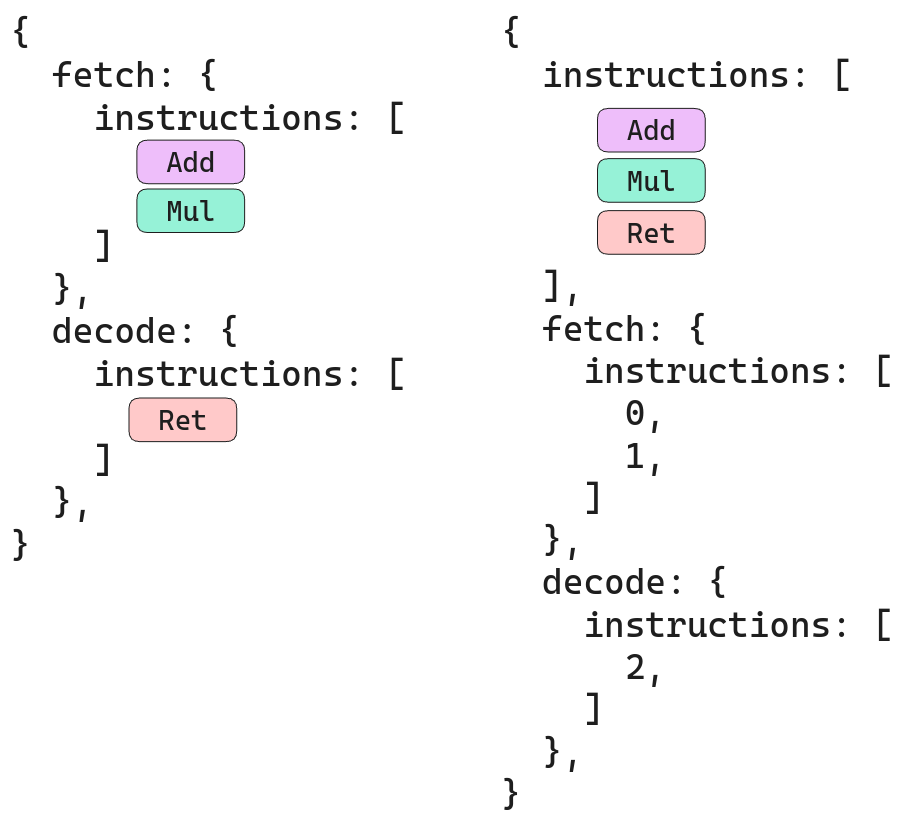
\includegraphics[width=10cm]{obrazky-figures/impl/json_normalization.png}
    \caption{Zjednodušený stav procesoru (vlevo) a jeho normalizovaná verze (vpravo).} 
    \label{json_norm}
\end{figure}

\subsection{HTTP Server}
% Validace, optimalizace (gzip), návrh endpointů
% paralelní
% timeout

Server je implementovaný za pomocí knihovny \emph{Undertow}\footnote{\url{https://undertow.io/}}.
Tato knihovna poskytuje vcelku jednoduché rozhraní pro paralelní obsluhu HTTP požadavků a definici zdrojů (\emph{endpointů}).
Obsluha požadavku je přesunuta do pracovního vlákna, takže obsluha je neblokující.

Všechny endpointy využívají obecnou třídu pro zpracování těla POST požadavku ve formátu JSON, vyvolání daného kódu pro obsluhu a odeslání odpovědi.

HTTP server má konfigurovatelnou adresu (host a port), dobu po které dojde k~vypršení požadavku a přepínač pro použití komprese zip v~odpovědi.

Každý endpoint je definován svou cestou (např. \texttt{/compile}), obsluhovací metodou a datovým typem vstupu a výstupu.
Obsluhovací metoda kontroluje přítomnost povinných parametrů a vykoná aplikační logiku.
Metoda by měla korektně pracovat s~očekávanými chybami a vrátit chybovou hodnotu, která v~daném kontextu dává smysl. 

Neobsloužené výjimky jsou zachyceny serverem a vyřešeny generickou chybovou hláškou, aby nedošlo k~pádu aplikace. 

\subsection{Rozhraní příkazové řádky}
% využití (automatizace)

Rozhraní příkazové řádky nabízenou funkcionalitou odpovídá HTTP serveru.
Místo předávání argumentů v~těle POST požadavku se konfigurace specifikuje soubory.
Všechny parametry rozhraní jsou uvedeny v~příloze \ref{simArgs}.

\subsection{Integrace s~GCC}
% json, params, error reporting

Pro účely překladu programů definovaných v~jazyce C do jazyka RISC-V assembleru HTTP server poskytuje endpoint \texttt{/compile}.
Samotný překlad programu je uskutečněn třídou \texttt{GccCaller}, která poskytuje rozhraní pro volání kompilátoru GCC\footnote{\url{https://gcc.gnu.org/}}.

Proces překladu spočívá ve spuštění nového procesu, který vykoná program GCC s~určitými přepínači (\emph{flags}) a uživatelem zadaným kódem.
Standardní vstup, standardní výstup a standardní chybový výstup procesu jsou přesměrovány do paměti objektu \texttt{GccCaller}.
Návratová hodnota procesu vypovídá o~úspěchu překladu.

Cesta programu GCC je konfigurovatelná při spuštění serveru.
Dále je konfigurovatelná úroveň optimalizace programu.
Povoleny jsou přepínače \texttt{-O0}, \texttt{-O2}, \texttt{-O3} a \texttt{-Os}.
Výčet všech použitých přepínačů se nachází v~tabulce \ref{gccFlags}.

\begin{table}[]
\begin{tabular}{|l|p{8cm}|}
\hline
Přepínač                        & Význam                                                                \\ \hline\hline
\texttt{-xc}                             & Překlad jazyka C (nelze odvodit z~přípony souboru)                    \\ \hline
\texttt{-g} & Mapování řádků jazyka C do assembleru \\ \hline
\texttt{-march=rv32imfd}                 & Definice architektury a rozšíření M, F, D                             \\ \hline
\texttt{-mabi=ilp32d}                    & Generování funkcí s~ABI předávající argumenty registry                \\ \hline
\texttt{-o /dev/stdout}                  & Výstup na standardní výstup                                           \\ \hline
\texttt{-S}                              & Výstup ve formě assembleru                                            \\ \hline
\texttt{-fcf-protection=none}            & Vypnutí bezpečnostních ochran skokových instrukcí                     \\ \hline
\texttt{-fno-stack-protector}            & Vypnutí ochrany proti přetečení bufferů                               \\ \hline
\texttt{-fno-asynchronous-unwind-tables} & Vypnutí generování dat pro obsluhu výjimek                            \\ \hline
\texttt{-mno-explicit-relocs}            & Vypnutí relokace symbolických adres (operátory \texttt{\%hi()} a \texttt{\%lo()})       \\ \hline
\texttt{-ffunction-sections}             & Vytvoření zvláštní sekce pro každou funkci                            \\ \hline
\texttt{-fdata-sections}                 & Vytvoření zvláštní sekce pro každý datový objekt                      \\ \hline
\texttt{-fno-dwarf2-cfi-asm}             & Snížení šumu v~generovaném kódu                                       \\ \hline
\texttt{-finhibit-size-directive}        & Snížení šumu v~generovaném kódu                                       \\ \hline
\texttt{-mstrict-align}                  & Zabránění generování nezarovnaných paměťových přístupů                \\ \hline
\texttt{-nostdlib}                       & Zákaz využití standardní knihovny jazyka C                            \\ \hline
\texttt{-fdiagnostics-format=json}       & Výstup chyb ve formátu JSON                                           \\ \hline
\texttt{-fPIE}                           & Generování pozičně nezávislého kódu (position-independent code)       \\ \hline
\texttt{-fno-plt}                        & Zákaz generování nepřímých skoků pomocí PLT (Procedure Linkage Table) \\ \hline
\end{tabular}
\caption{Jednotlivé přepínače pro překlad. K~těmto přepínačům je ještě přidán přepínač pro žádanou úroveň optimalizace. Většina přepínačů pomáhá generovat čitelnější kód vhodnější ke zpracování simulátorem.}
\label{gccFlags}
\end{table}

Kompilace každého objektu do zvláštní sekce znemožní optimalizace využívající relativní polohu kódu a dat, což je žádoucí vzhledem k~tomu, že data budou v~simulátoru alokována na jinou než předpokládanou pozici.

Existence \texttt{memcmp} a \texttt{memset} je do GCC vestavěna a nelze zabránit generování jejich volání.
Rovněž se mi nepodařilo zakázat volání jiných vestavěných funkcí jako například \texttt{\_\_builtin\_popcount(n)}.
Endpoint tedy programy s~těmito voláními zpracovává a nehlásí chybu, i když s~takovým programem simulátor není schopen pracovat.

% filter
Výstup v~podobě assembleru obsahuje velké množství informací, které jsou pro simulátor nadbytečné a navíc snižují čitelnost kódu.
Proto výstup překladače prochází filtrem, který odstraní nedůležité direktivy, návěstí a data.
Výstupem je tak podstatně čitelnější kód, obsahující pouze relevantní údaje.
Příklad celé transformace je uveden v~\ref{asmFilter}.

\begin{figure}[ht]
     \centering
     \begin{subfigure}[b]{0.4\textwidth}
         \centering
         \begin{lstlisting}
int f(int x) {
    return 2 * x;
}
\end{lstlisting}
         \caption{Vstupní program v~jazyce C.}
         \label{asmFilterA}
     \end{subfigure}
     \hfill
     \begin{subfigure}[b]{0.6\textwidth}
         \centering
         \begin{lstlisting}
  .file "<stdin>"
  .option pic
  .attribute arch, "rv32i2p1_m2p0_f2p2_d2p2_zicsr2p0"
  .attribute unaligned_access, 0
  .attribute stack_align, 16
  .text
  .section .text.f,"ax",@progbits
  .align 2
  .globl f
  .type f, @function
f:
  slli  a0,a0,1
  ret
  .ident "GCC: (Ubuntu 12.3.0-1ubuntu1~22.04) 12.3.0"
  .section .note.GNU-stack,"",@progbits

\end{lstlisting}
         \caption{Assembler před filtrovacím krokem.}
         \label{asmFilterB}
     \end{subfigure}
          \hfill
     \begin{subfigure}[b]{0.4\textwidth}
         \centering
         \begin{lstlisting}
f:
  slli    a0,a0,1
  ret
\end{lstlisting}
         \caption{Kód po filtrování.}
         \label{asmFilterC}
     \end{subfigure}
        \caption{Kroky zpracování programu jazyka C.}
        \label{asmFilter}
\end{figure}

% filter inner workings
Filtr nejdříve rozdělí text na sekce a smaže ty, které nepopisují kód ani data.
Text je dále rozdělen na jednotlivé řádky a řádek assembleru je spojen s~odpovídajícím řádkem programu v~C\footnote{Tento krok souvisí s~vizualizací vysvětlenou v~kapitole \ref{codeEditorPage}.}. 
Dalším krokem je přečtení instrukcí a sběr používaných návěstí.
Na základě této informace jsou smazány všechny direktivy, na které neodkazuje žádné používané návěstí.

Výsledkem je čistý program s~dodatečnou informací o~vztahu mezi řádky původního programu a přeloženého assembleru.
Mapování je využito v~editoru kódu webové aplikace.

\chapter{Implementace webové aplikace}
\label{implementaceweboveaplikace}
% Next.js

Požadavky na aplikaci ze sekce \ref{webAppDesign} lze splnit mnoha způsoby.
Vzhledem k~rozsahu aplikace budu volit z~rámcových řešení pro webové aplikace.
Faktory při výběru frameworku byly popularita, kvalita dokumentace, osobní zkušenost a dispozice knihoven.

Pro implementaci jsem zvolil JavaScriptový framework Next.js\footnote{\url{https://nextjs.org/}}.
Jedná se o~v~současnosti nejrozšířenější způsob psaní aplikací s~knihovnou React.
Jeho hlavními znaky jsou úzké propojení se serverovou stranou a hybridní přístup k~renderování stránek.

% Typescript
Next.js aplikace je možné psát buď v~jazyce JavaScript nebo TypeScript.
Kvůli rozsahu aplikace jsem zvolil TypeScript s~předpokladem, že typové informace usnadní implementaci.

Příloha \ref{gallery} obsahuje více obrázků webové aplikace.

\section{Logika aplikace}
% redux, persistence, global state

Z~pohledu klientské aplikace interaktivní simulace spočívá v~následujících krocích: 
\begin{enumerate}
    \item kontaktovat simulační server s~požadovanou konfigurací,
    \item získat a uložit odpověď (nový stav procesoru),
    \item zpřístupnit nový stav všem relevantním komponentům,
    \item spustit renderování komponentů (prezentace).
\end{enumerate}
Tento postup se opakuje při každém kroku simulace.
Pro implementaci práce se stavem jsem zvolil knihovnu pro správu globálního stavu \emph{Redux}\footnote{\url{https://redux.js.org/}}.

Redux poskytuje rámcové řešení pro popis stavu, přechodů mezi stavy a selektory.
Redux konceptualizuje globální stav jako objekt, který mezi stavy přechází funkcemi zvanými \emph{reducers}.
Jedná se o~čisté funkce, knihovna se zde inspirovala funkcionálním programováním.

Přístup k~části stavu je zprostředkován \emph{selektory}.
Selektor je funkce, která ze stavu vybírá jeho podmnožinu. 
Díky použití selektorů a přechodů je možné určit datové závislosti mezi komponentami a globálním stavem a znovu renderovat pouze ty komponenty, jejichž data byla změněna.

% persist, migrations
Knihovna mi dovolila velmi jednoduše implementovat perzistenci stavu.
Díky tomu je konfigurace zachována mezi sezeními.
Důležité je při každé změně schématu globálního stavu definovat \emph{migraci}, aby aplikace nepracovala se starým, neočekávaným formátem dat.
Tato technika je běžně používaná v~databázích.

% DX - chrome extension
Další přidanou hodnotou je vývojové rozšíření prohlížeče, které umožňuje prohlížet všechny přechody mezi stavy na časové ose.
Detailní náhled stavu umožňuje zobrazit změny z~posledního přechodu (\emph{diff}), nebo aplikaci do zvoleného stavu přenést.
Tyto funkce jsou umožněny transakční/funkcionální architekturou.
Možnost detailně prohlížet stav aplikace mi několikrát usnadnilo řešení problémů.

Globální stav se organizuje do celků s~názvem \emph{slice}.
Jeden slice se má týkat stavu jedné funkcionality.
V~aplikaci jsou 4 slicy:
\begin{itemize}
    \item \texttt{isaSlice} -- ukládá konfigurace procesoru a aktivní konfiguraci,
    \item \texttt{cpustateSlice} -- ukládá aktuální stav interaktivní simulace,
    \item \texttt{compilerSlice} -- obsahuje stav editoru kódu,
    \item \texttt{simConfigSlice} -- obsahuje aktuální simulovanou konfiguraci a kód.
\end{itemize}

% Problém dvou implementací validace vstupů
Jedním z~problémů na který jsem narazil při implementaci byla dvojí implementace kontrola oborů hodnot parametrů.
Jedna implementace se nacházela v~serverové části a druhá ve webové části kódu.
Udržení implementací v~synchronizovaném stavu probíhalo manuálně, což je práce náchylná k~chybám.

\section{Komunikace se serverem}
% server props, caching

Výsledkem překladu projektu ve frameworku Next.js je serverová aplikace a staticky vygenerované zdroje (HTML, CSS, JS).
Prvním požadavkem na server se stáhne statický základ stránky, poté na straně klienta proběhne inicializace Reactu (hydratace) a UI se stává interaktivním.
Veškeré další požadavky na server včetně navigace probíhají přes webové \texttt{fetch API}.

% robots.txt? sitemap?
% https://nextjs.org/docs/app/api-reference/file-conventions/metadata
Webový server kromě stránek, stylů a skriptů nabízí dva statické zdroje: příklady kódů a strukturovaný popis instrukcí RISC-V.
Oba objekty jsou poskytovány přes HTTP API ve formátu JSON.

% sim proxy
První verze řešení využívala přímé volání simulačního serveru, které muselo být nasazeno na adrese dostupné klientovi.
Finální řešení přístup klienta ke službám simulačního serveru zprostředkovává přes webový server, který pracuje jako \emph{proxy}.
Při nasazení je tedy zapotřebí konfigurovat jedinou adresu, na které klient získá i webové rozhraní i simulační služby.
Celá komunikace je nastíněna na obrázku \ref{diagramApiComms}.

\begin{figure}[ht]
    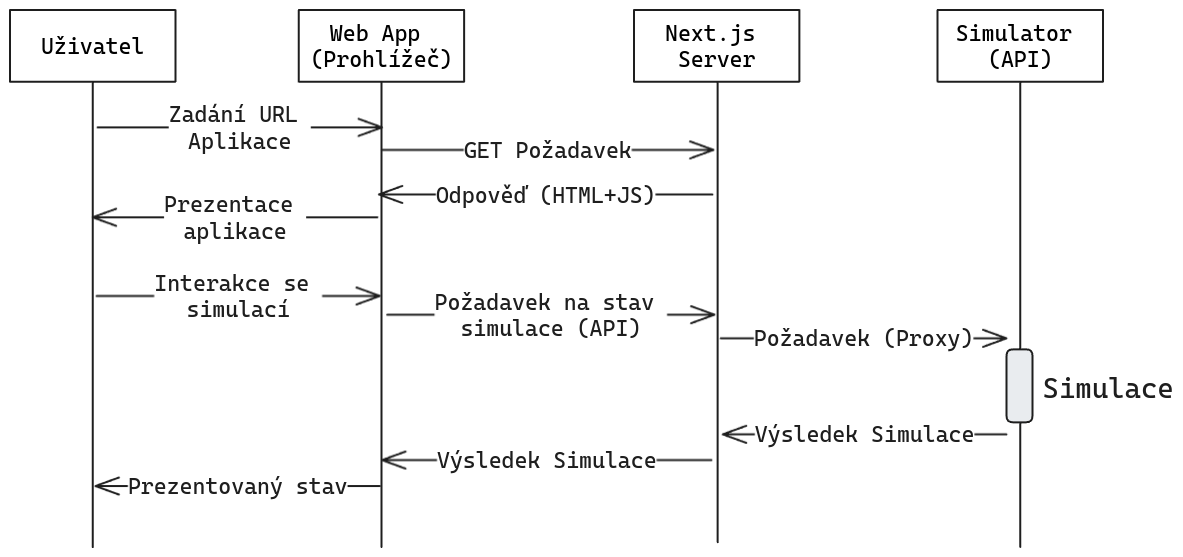
\includegraphics[width=\textwidth]{obrazky-figures/impl/apicomms.png}
    \caption{Sekvenční diagram komunikace prohlížeče a serveru.}
    \label{diagramApiComms}
\end{figure}

Odpověď simulačního serveru je uložena do globálního stavu, čímž spustí renderování nového stavu simulace.
Redux umožňuje narušit funkcionální povahu přechodů mezi stavy a při přechodu provést HTTP dotaz. 

% caching, prefetching
Framework Next.js ve výchozím nastavení poskytuje mnoho optimalizací.
Mezi nejvýznamější patří caching a prefetching zdrojů.
Výsledkem prefetchingu odkazů zobrazených na stránce ve výsledku znamená okamžitou navigaci mezi stránkami. 

\section{Stránky}
% nebo "pohledy/views"
% settings, layouts, side menu

Aplikace se skládá z~osmi hlavních pohledů.
V~následujících podsekcích rozvedu některé z~jednotlivých stránek, jejich účel a způsob implementace.

% ostatní stránky, moc krátké na podsekci

Stránka nastavení poskytuje pouze tři funkce -- smazaní lokálního úložiště, export dat a výběr mezi světlou a tmavou barevnou paletou.

\subsection{Simulační okno}
\label{simWindow}

% todo welcome popup

Simulační okno je jádrem celé aplikace.
Je zároveň nejsložitější částí aplikace.
Okno obsahuje schéma procesoru a dva samostatné prvky: horní ovládací menu a pravou lištu.

% posuvné okno
% bloky, trasy, zvětšování
Prostřední část okna je věnována schématu procesoru.
Vedle sebe zde leží rozmístěny jednotlivé obdélníkové bloky, které odpovídají blokům v~simulátoru.
Mezi bloky vedou spoje, které naznačují jejich souvislost.

Všechny bloky sdílejí ovládací prvky.
Blok jednotky fetch je uveden na obrázku \ref{simblock_figure}.
V~horní části vedle názvu bloku (1) se nachází tlačítko (4) vyvolávající vyskakovací okno s~detailem bloku.
Pod ním je několik nejdůležitějších informací o~aktuálním stavu (2).
Potažením pravého dolního rohu (5) se dá změnit velikost bloku.
Rozmístění bloků je k~této změně responzivní.
Zbytek plochy je specifický pro každý druh bloku.
Nejčastěji obsahuje seznam instrukcí (3), které se v~bloku momentálně nacházejí.

\begin{figure}[hbtp]
    \begin{center}
        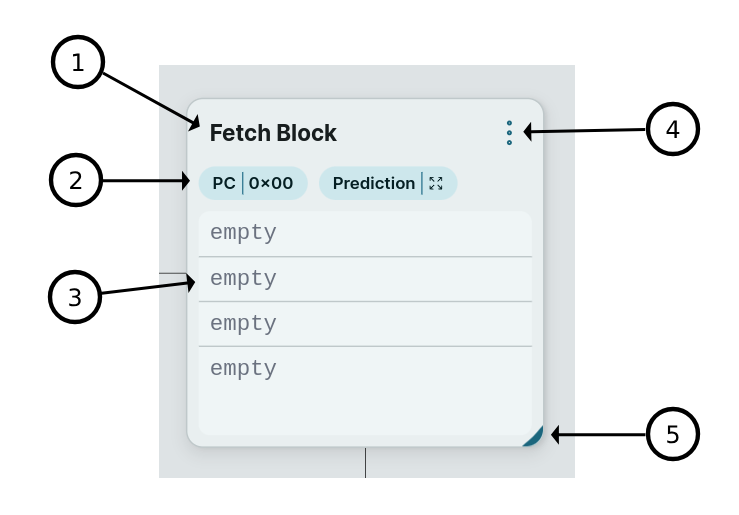
\includegraphics[width=11cm]{obrazky-figures/impl/simblock.png}
    \end{center}
    \caption{Reprezentace bloku Fetch.}
    \label{simblock_figure}
\end{figure}

Celý pohled na procesor lze posouvat a přibližovat.
Technicky je této možnosti docíleno sledováním pohybu myši nad oknem a přepočítáváním odsazení všech bloků od počátku souřadného systému.

% ovládání simulace, zkratky, automatika
Simulaci je možno ovládat jak myší, tak i klávesnicí.
Pro ovládání myší je v~horní části obrazovky menu s~tlačítky umožňující krok v~simulaci dopředu nebo zpět, skok na začátek nebo konec simulace.
Stejné možnosti jsou k~dispozici klávesovými zkratkami.
Druhé menu v~horní části obrazovky nabízí automatické krokování simulace.
Prodleva mezi kroky je nastavitelná v~textovém poli.

% detaily bloků a instrukcí
Schématický pohled na stav simulace poskytuje celkový přehled, nemůže ale zobrazit všechny detaily, které jsou k~dispozici.
K~tomu slouží vyskakovací náhledy.
Kliknutím na blok nebo instrukci se objeví okno, které v~tabulkové formě poskytuje dostupné informace.
Pro instrukce se jedná o~časové známky důležitých aktivit (fetch, execute), hodnoty paramtetrů a příznaky (například zda je instrukce spekulativní, či zda jsou všechny parametry připraveny k~vykonání).
Detaily bloků jsou specifické pro každý blok.
Například detail bloku hlavní paměti (na obrázku \ref{mainmemory_popup_figure}) ukazuje všechny ukazatele v~programu, jejich adresy a větší znázornění celé paměti.

\begin{figure}[hbtp]
    \begin{center}
        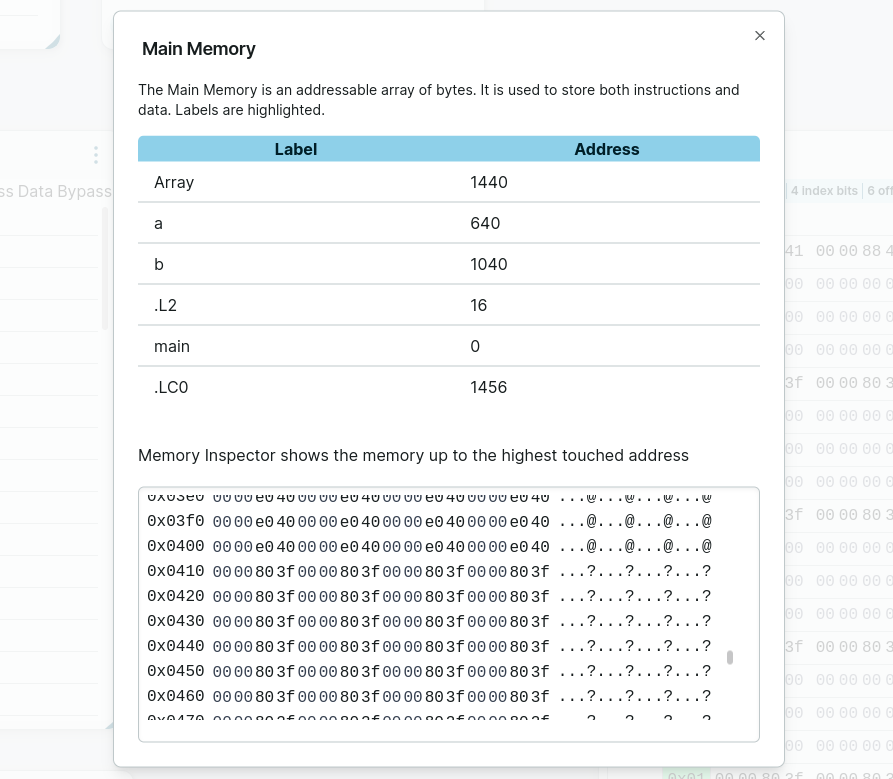
\includegraphics[width=12cm]{obrazky-figures/impl/mainmemory_popup.png}
    \end{center}
    \caption{Detail bloku hlavní paměti.}
    \label{mainmemory_popup_figure}
\end{figure}

% přejetí nad instrukcí nebo registrem
% hover bubliny
Po najetí na instrukci nebo registr se zvýrazní všechny jejich výskyty v~ostatních blocích.
Tato funkce je velmi užitečná pro zorientování ve stavu simulace. 
Implementace je rozvedena v~sekci \ref{optimRender}, kde je popsán i proces její optimalizace.
Po najetí myší na parametr instrukce se také objeví bublina s~jeho hodnotou.
U~registru se navíc objeví informace o~jeho přejmenování. 

% lišta - statistiky, log
Lišta na pravé straně zobrazuje vybrané statistiky a log.
Lišta má dva stavy: výchozí a expandovaný.
V~expandovaném stavu vzniká místo pro více statistik a textu zpráv z~logu.
Ke zobrazení jsem vybral statistiky, které považuji za nejrelevantnější při simulování: počet taktů, počet vydaných instrukcí, IPC a úspěšnost predikce skoků.
Kompletní statistiky jsou zobrazeny na zvláštní stránce (viz sekce \ref{statsPage}).
Každá zpráva v~logu má svou časovou známku (takt, kdy zpráva vznikla).
Kliknutím na číslo zprávy se simulace do tohoto taktu přenese.

% obrázek s očíslovanými šipkami na prvky

\subsection{Editor kódu}
\label{codeEditorPage}

Editor (na obrázku \ref{codeeditor_figure}) nabízí lištu s~akcemi a dvě textová pole.
V~levém sloupci lze ovládat kompilaci.
Prostřední okno slouží k~psaní kódu v~jazyce C, pravé okno zobrazí výsledek překladu.

Textová pole jsou implementována za pomocí knihovny CodeMirror\footnote{\url{https://codemirror.net/5/}}.
Tato knihovna poskytuje dobré uživatelské rozhraní pro editaci kódu, například běžné zkratky, zvýraznění syntaxe, zobrazení varování, očíslování řádků a další.
Důležitá byla i možnost vytvořit vlastní rozšíření.

\begin{figure}[hbtp]
    \begin{center}
        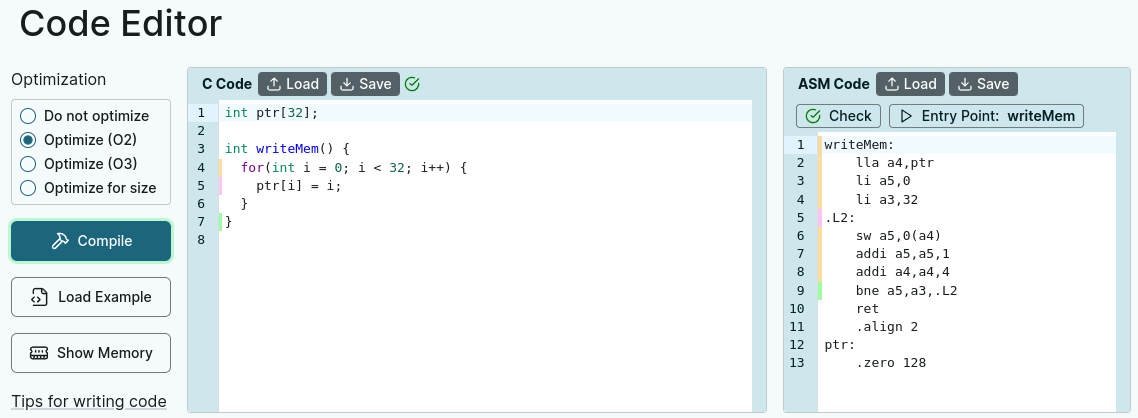
\includegraphics[width=15cm]{obrazky-figures/impl/codeeditor.png}
    \end{center}
    \caption{Editor kódu s kompilátorem.}
    \label{codeeditor_figure}
\end{figure}

Souvislost částí kódu je naznačena barevným páskem na levé straně textového pole.
Najetím myší na skupinu řádků se vztah vyznačí výrazněji.
Při najetí myší na instrukci (obrázek \ref{codeeditorhover_figure}) se také objeví vyskakovací okno s~informací o~argumentech instrukce.

\begin{figure}[hbtp]
    \begin{center}
        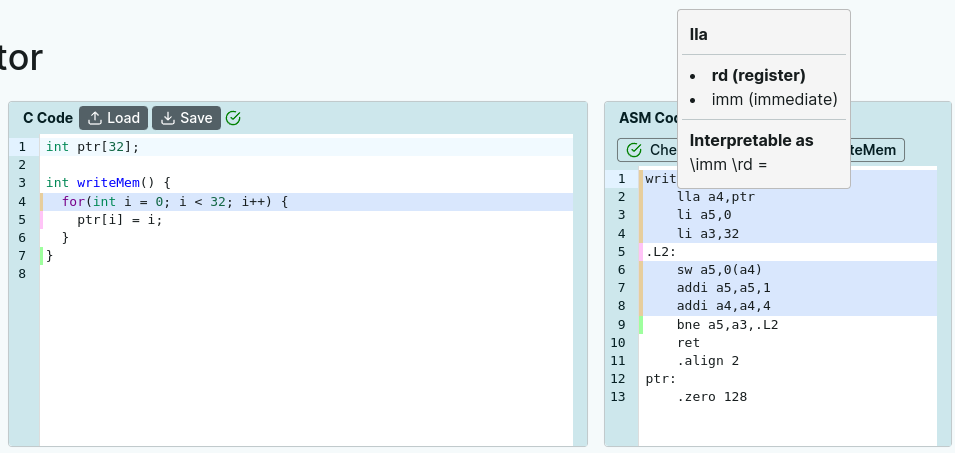
\includegraphics[width=15cm]{obrazky-figures/impl/codehover.png}
    \end{center}
    \caption{Vzhled editoru při najetí myší na instrukci.}
    \label{codeeditorhover_figure}
\end{figure}

O~vyznačení chyb v~textovém poli se stará knihovna CodeMirror, chyby je ale nutné z~výstupu simulátoru převést do správného formátu.
Chybná část kódu je podtržena, po najetí na oblast myší je zobrazena chybová zpráva (viz obrázek \ref{codeerrors}).
Zpráva o~chybách nebo úspěchu překladu se také objevuje v~rohu obrazovky.

\begin{figure}
     \centering
     \begin{subfigure}[b]{0.56\textwidth}
         \centering
         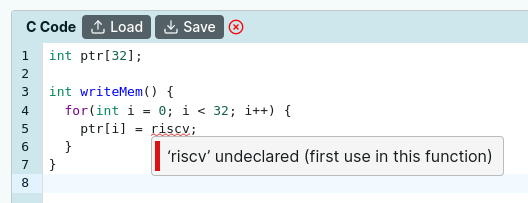
\includegraphics[width=\textwidth]{obrazky-figures/impl/c_error.png}
         \caption{Chyba v~programu jazyka C. Hlášení jsou předávána z~kompilátoru GCC.}
         \label{fig:codeerrors1}
     \end{subfigure}
     \hfill
     \begin{subfigure}[b]{0.42\textwidth}
         \centering
         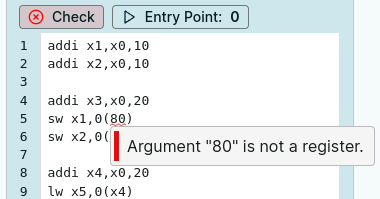
\includegraphics[width=\textwidth]{obrazky-figures/impl/asm_error.png}
         \caption{Chyba v~Assembleru RISC-V. Hlášení pochází z~vlastního kompilátoru assembleru (viz sekce \ref{parsingAsmCode}).}
         \label{fig:codeerrors2}
     \end{subfigure}
        \caption{Zobrazení chyb v~editoru.}
        \label{codeerrors}
\end{figure}


V~neposlední řadě je zde možné zvolit vstupní bod programu.
Vstupním bodem může být první instrukce, nebo libovolné návěstí.

\subsection{Konfigurace paměti a procesoru}
% formuláře

Konfigurace paměti (simulačních dat) a procesoru jsou formulářové stránky.
Obsahují velké množství vstupních textových polí s~názvem, vysvětlivkami a validací.
Formuláře kopírují strukturu konfigurace simulátoru.

Logika formulářů je implementována pomocí knihovny \emph{React Hook Form}.
Schéma formuláře je definováno objekty validační knihovny \emph{Zod}.

Vstupní textové pole a přepínač (\emph{radio input}) jsou znovupoužitelné komponenty.

Konfigurace procesoru je rozdělena do záložek, které všechny možnosti organizují do kategorií.
V~horní části obrazovky je možné přepínat mezi uloženými konfiguracemi, nebo založit konfiguraci novou.
Zvláštním prvkem formuláře je \uv{podformulář} pro definice funkčních jednotek.

Konfigurace paměti umožňuje přidávat, upravovat a mazat datové objekty.
Datový objekt má jméno, zarovnání, datový typ a samotná data.
Data je možné definovat několika způsoby:
\begin{enumerate}
    \item explicitním výčtem prvků,
    \item opakováním konstanty (po vzoru \texttt{memset}),
    \item rozsahem náhodných prvků (např. 32 čísel v~rozsahu 0-15).
\end{enumerate}
Formulář nemá plnou vyjadřovací schopnost -- jsou konfigurace paměti, které lze definovat pouze ručně psanou definicí ve formátu JSON.
Takové definice ale lze do webové aplikace importovat a pracovat s~nimi.

\subsection{Statistiky}
\label{statsPage}

Jak bylo zmíněno v~sekci o~hlavním simulačním okně (\ref{simWindow}), nejdůležitější statistiky jsou zobrazeny v~boční liště při simulaci.
Detailnější pohled na sbírané statistiky je k~dispozici ve speciálním okně.

Stránka je organizovaná do karet podle kategorií statistik.
Tři karty jsou ukázány na obrázku \ref{stats_screenshot}.
Modul na pravé straně ukazuje statistiky ke konkrétní instrukci v~podobě \emph{teplotní mapy}.
Lze v~něm přepnout mezi pohledem na úspěšnost nalezení dat v~cache a podílem vydaných instrukcí v~průběhu programu.

\begin{figure}[hbtp]
    \begin{center}
        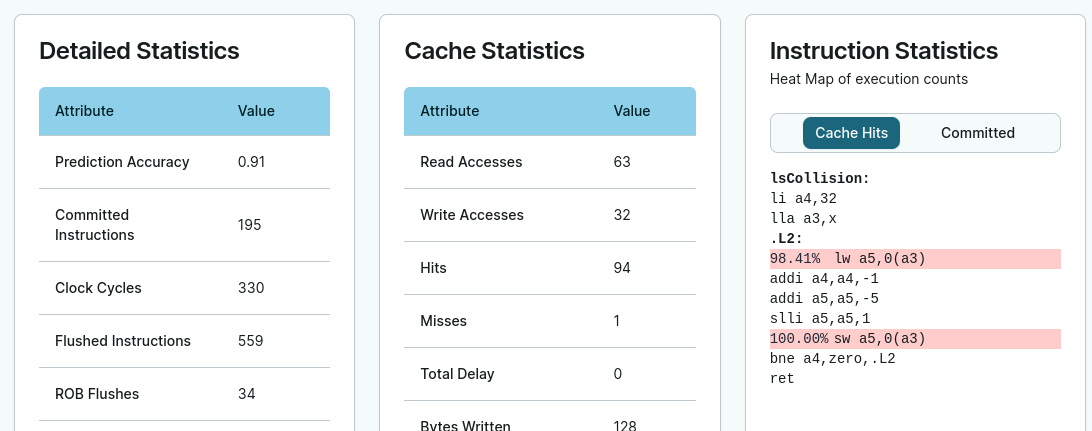
\includegraphics[width=15cm]{obrazky-figures/impl/stats.png}
    \end{center}
    \caption{Výřez obrazovky statistik poskytovaných na vyhrazené stránce.}
    \label{stats_screenshot}
\end{figure}

\subsection{Edukativní stránky}

Součástí aplikace je krátký informativní úvod do architektury RISC-V.
Tento text vysvětluje základní informace o~registrech a konvenci volání, což může být užitečné pro někoho, kdo má zkušenosti s~assemblerem, ale ne konkrétně s~RISC-V.
Pro hlubší porozumění jsou poskytnuty odkazy na detailnější materiály.

Jiná edukativní stránka se věnuje přehledu architektury procesoru.
Každému důležitému komponentu je věnována krátká sekce.

Poslední stránkou je nápověda.
Ta uvádí zkratky, kterými je možné simulaci ovládat.
Obsahuje také tipy pro psaní kódu pro simulátor, včetně jeho specifik a odchylek.

\section{Design a použitelnost}
% barevné schéma, layout a hierarchie, nápovědy
% shad/cn, radix, tailwindcss, lucide icons
% vizualizace (prediktorů)

% component libraries
Mnoho komponentů (například formuláře, nebo karty objevující se po přejetí myší a vyskakovací okna) je implementovaných pomocí knihoven předpřipravených komponentů.
Tyto komponenty zajišťují dobrou úroveň dostupnosti a správné chování napříč zařízeními.
Zároveň umožňují detailní úpravu podle požadavků programátora.

Komponenty jsou stylovány kombinací CSS a stylovací knihovny \emph{TailwindCSS}\footnote{\url{https://tailwindcss.com/}}, která poskytuje obecné stylovací třídy.
Na stránkách jsou využity sémantické značky HTML (například \texttt{<section>}, \texttt{<nav>}, které přesněji vyjadřují význam částí stránky.

% barevná paleta, dark mode
Navrhnout vhodnou a funkční barevnou paletu je těžký designový úkol, který byl přenechán nástroji \emph{Material Theme Builder}\footnote{\url{https://m3.material.io/theme-builder}}.
Algoritmus od společnosti Google, který se používá v~operačním systému Android, generuje vizuálně zajímavou paletu splňující požadavky na kontrast.
Paleta má také variantu pro tmavý režim rozhraní.
Obrázek \ref{lightanddarkmode} ukazuje porovnání světlé a tmavé palety rozhraní.
% TODO https://material.io/blog/science-of-color-design

% Tab navigation
Zvláštní důraz byl kladen na možnost ovládat celou aplikaci klávesnicí.
Motivací bylo dát všem uživatelům tuto možnost, neméně důležité ale bylo udělat maximum pro dobrou dostupnost aplikace.
Rozhraní simulace obsahuje velké množství interaktivních prvků (dlouhé tabulky instrukcí), což může učinit navigaci na konkrétní prvek zdlouhavé.
Tento nedostatek není zcela vyřešen, prázdná pole jsou ale při navigaci ignorována.

Zobrazení aplikace je optimalizováno pro všechny velikosti obrazovky.
Obrázek \ref{mobile_layout} jako příklad ukazuje rozložení stránky kompilátoru na mobilním zařízení (obrázek \ref{codeeditorhover_figure} ukazuje stejnou část rozhraní na široké obrazovce stolního počítače).
Prvky mají užší okraje a komponenty jsou uspořádány vertikálně.
Aplikaci je možné na mobilním zařízení úspěšně používat, omezení malé dotykové obrazovky ale snižuje pohodlí.

\begin{figure}[hbtp]
\centering
    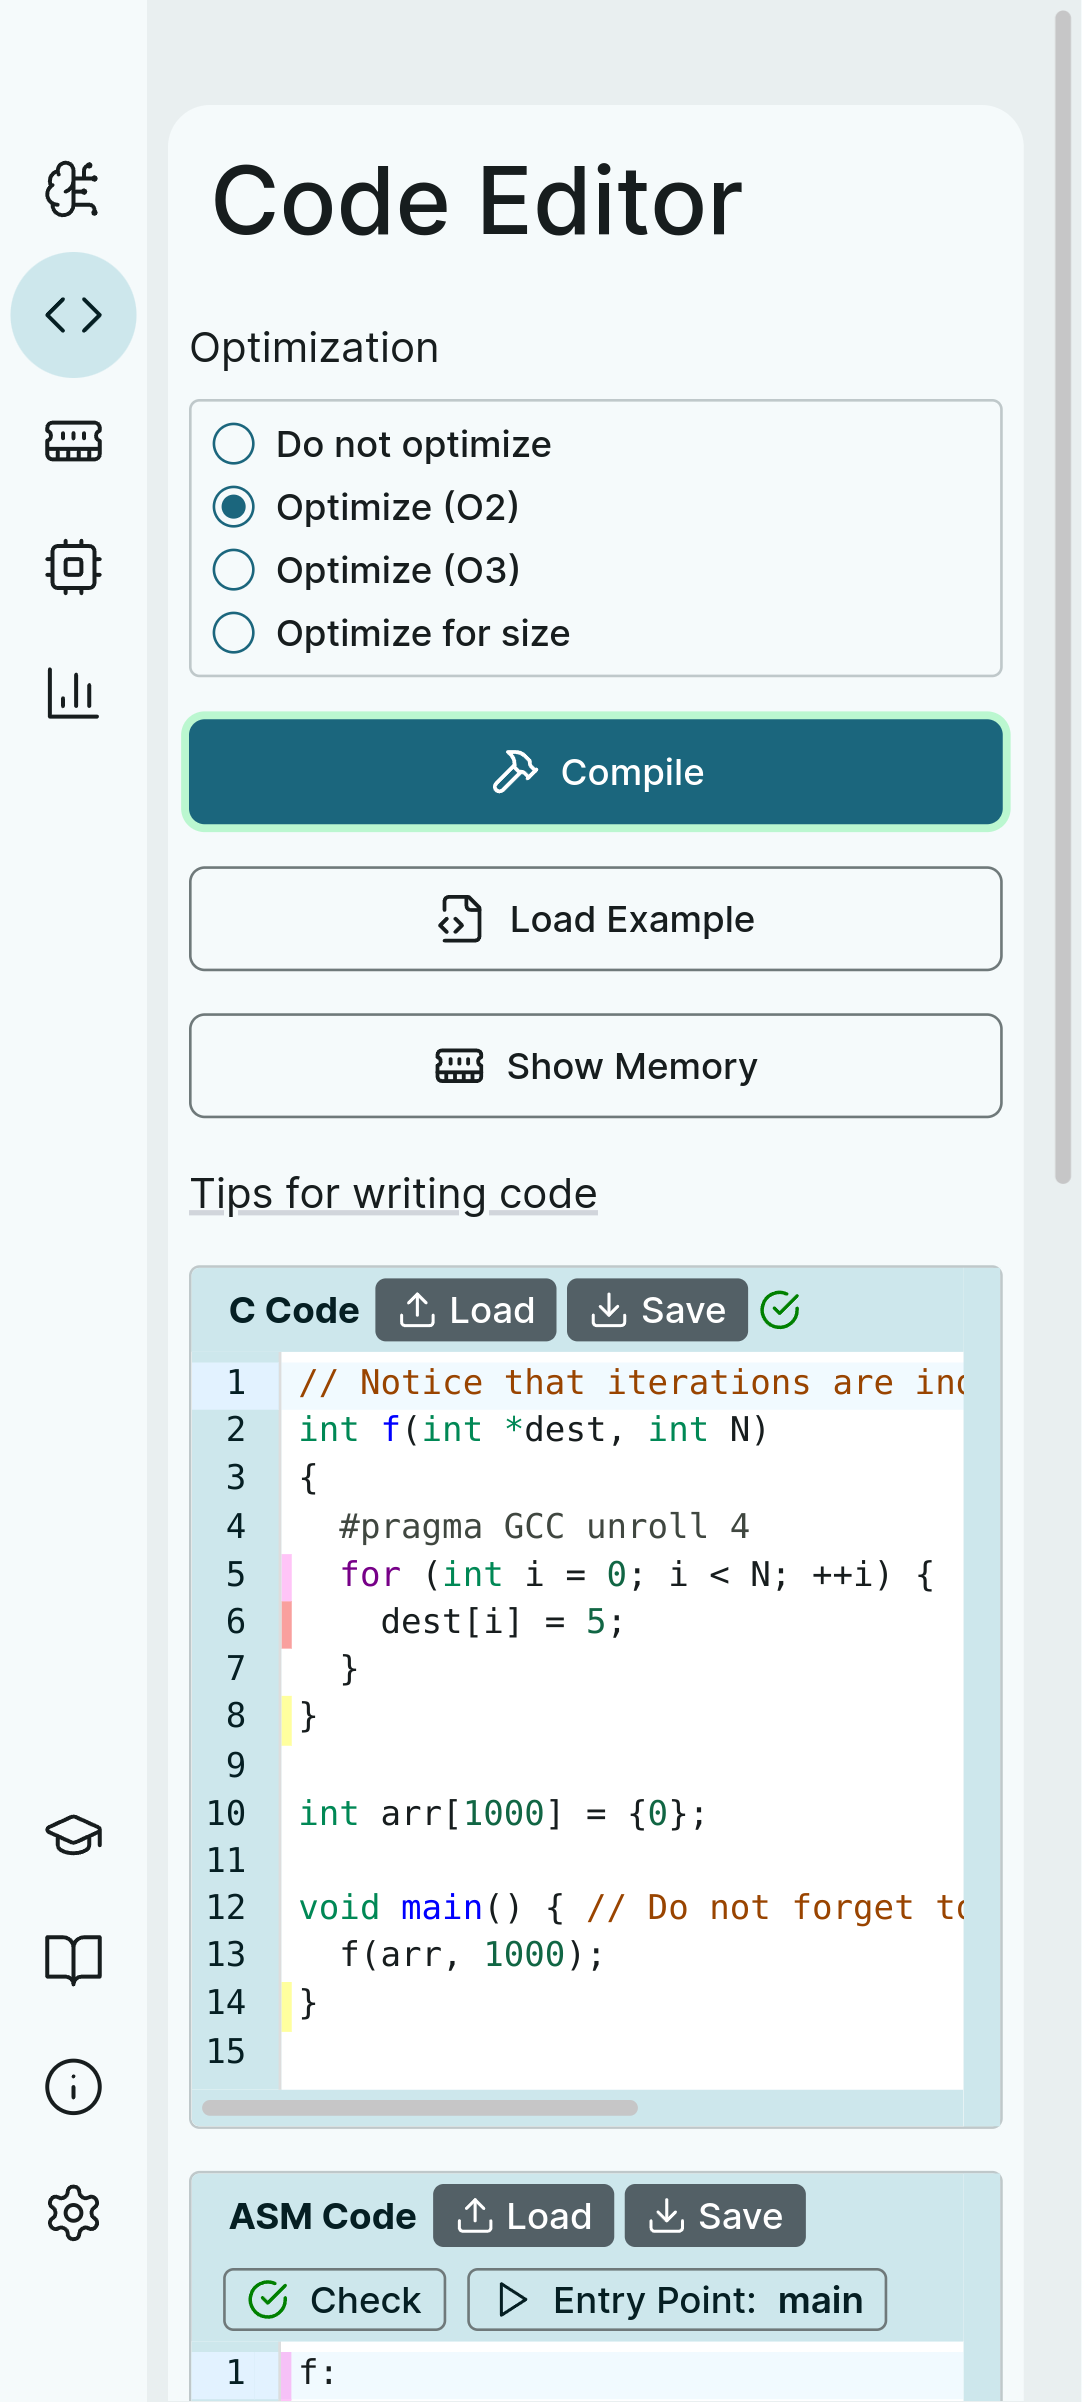
\includegraphics[width=9cm]{obrazky-figures/impl/mobile_layout_compiler.png}
    \caption{Pohled kompilátoru v~rozložení pro mobilní telefony.} 
    \label{mobile_layout}
\end{figure}



\begin{figure}
     \centering
     \begin{subfigure}[b]{0.49\textwidth}
         \centering
         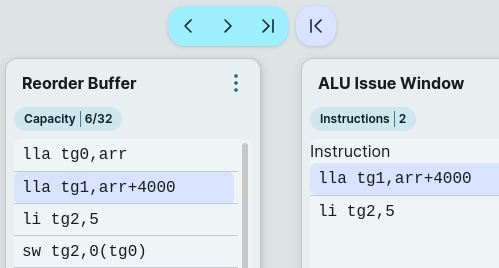
\includegraphics[width=\textwidth]{obrazky-figures/impl/lightmode.png}
         \caption{Simulátor ve světlém režimu rozhraní.}
         \label{fig:lightmode}
     \end{subfigure}
     \hfill
     \begin{subfigure}[b]{0.49\textwidth}
         \centering
         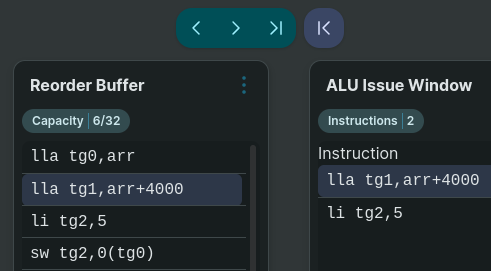
\includegraphics[width=\textwidth]{obrazky-figures/impl/darkmode.png}
         \caption{Simulátor v~tmavém režimu rozhraní.}
         \label{fig:darkmode}
     \end{subfigure}
        \caption{Světlá a tmavá varianta palety barev.}
        \label{lightanddarkmode}
\end{figure}

\subsection{Komponenty rozhraní, React}
% nextjs

Rozhraní je členěno do hierarchie komponentů.
Většina komponentů je definovaných ve zvláštním souboru, ale některé příliš specifické komponenty se nachází v~souboru společně s~místem použití.

Při návrhu uživatelského rozhraní pomocí React komponentů byly dodržovány zásady jediné odpovědnosti (SRP), což pomohlo udržet každou komponentu co nejvíce oddělenou a specializovanou na svou úlohu.
Každá komponenta byla navržena s~definovaným účelem, rozhraním a funkcionalitou, což usnadňuje správu kódu a jeho budoucí rozšíření.
Komponenty jsou ve struktuře projektu organizovány podle stránek nebo účelu, ke kterému náleží.

Dalším důležitým principem byla znovupoužitelnost.
Některé komponenty jsou využívány v~různých částech aplikace a v~různých kontextech.
Příkladem je komponent pro zobrazení programu, který je využitý jak v~simulačním tak statistickém okně.

\subsection{Optimalizace renderování}
\label{optimRender}
% memo, dělení do komponentů
% profilování

% Přesun do css
% todo české uvozovky
Důležitou součástí rozhraní simulace je interaktivní zvýraznění všech výskytů instrukce nebo registru napříč bloky.
První řešení informaci o~novém \uv{aktivním} prvku zapisovalo do globálního stavu.
Styl zvýraznění byl vypočítáván JavaScriptem, takže změna stavu spustila renderování \emph{celého} náhledu.
Tento přístup nebyl optimální a negativně se projevoval na responzivitě rozhraní.
Přejetím kurzoru napříč oknem se mohly vykonat i desítky událostí způsobujících renderování.

Řešením bylo přesunutí datové závislosti z~Reactu do CSS.
Jádro řešení zůstává stejné -- JavaScript stále naslouchá události najetí myši na instrukci a změny se stále zapisují do globálního stavu.
Důležitým rozdílem je, že změna stavu vyvolává změnu v~dynamicky generovaném kaskádovém stylu místo změny v~závislostech Reactu. 
Vyhodnocení CSS pravidel probíhá v~kódu prohlížeče, který je mnohem výkonnější.
Stylování probíhá pravidlem, které vybírá elementy na základě hodnoty jeho atributu (ID).
Po implementaci této optimalizace probíhá zvýrazňování okamžitě.

% virtual lists
% in extreme, 11700 DOM elements -> 6500 elements
Druhou významnou optimalizací bylo využití virtuálních rolovacích seznamů v~blocích, které zobrazují velké množství prvků.
Virtuální seznam využívá předpokladu, že většina prvků seznamu není zobrazených ve stejný okamžik.
Renderovány jsou jen ty prvky, které mají být v~daný okamžik viditelné.
Jestli má prvek být viditelný je vypočteno na základě velikosti prvků v~seznamu a velikosti rolovacího okna.

Implementace optimalizace se projevila významným snížením doby renderování, obzvlášť v~náhledu do hlavní paměti procesoru, který má velké množství elementů.
Při pokusu jsem naměřil pokles v~počtu HTML elementů na stránce z~11700 na ~6500.

\chapter{Testování, dokumentace a nasazení}
\label{testingchapter}
% formát kódu a komentářů (handbook sc fit)
% vývojové praktiky

V~této kapitole budou popsány okolní činnosti související s~vývojem aplikace.
Zejména se zaměří na testování simulátoru a webové aplikace.

%docs
% Java: 173 souborů, 10735 komentářů, 19577 kódu => cca 5545 bez hlaviček
% TS:   130 souborů, 4541 komentářů, 12073 kódu => cca 640 bez hlaviček
Celý projekt obsahuje asi 33\,000 řádků kódu (bez komentářů a prázdných řádků).
Velikost projektu je uvedena pro kontext množství komentářů: asi 6\,000 řádků (15\,000 včetně hlaviček souborů).
Při refaktorizaci simulátoru byl razantně zvýšen počet komentářů, jak v~hlavičkách funkcí a tříd, tak uvnitř kódu.
% todo spočítat počty komentářů

Během vývoje byl využit systém pro správu verzí \texttt{git}.
Kód byl před každým sloučením do hlavní větve prověřen vedoucím práce. 

V~projektu byl použit styl kódu z~příručky \emph{Handbook SC FIT} (příručky pro skupinu SC@FIT). 
Použití jasně definovaných pravidel pro úpravu kódu zajišťuje konzistenci a přehlednost kódu, která usnadňuje orientaci a úpravy pro současné i budoucí členy týmu.

\section{Testování simulátoru}
% Testování příkladů
% todo coverage

%todo pomohly mi logy při uživatelském testování

Během implementace simulátoru (sekce \ref{implSimulace}) byly intenzivně využívány jak existující testy, tak nově vytvořené testy, které byly postupně doplňovány.
Testy zvyšovaly důvěru ve správnost úprav i nových funkcí simulátoru.
Projekt v~současném stavu obsahuje více než 400 testů.
Pokrytí řádků kódu testy v~simulátoru je 83\%.
Pokrytí v~blocích simulátoru je 94\%.

Jednotkové testy (unit tests) testují izolované moduly.
Izolované testování jednotlivých tříd a systémů simulátoru bylo stěžejním pro úspěšnou implementaci.
Důkladněji testované byly moduly Cache, prediktory a překlad kódu.
Kód byl navrhován tak, aby byl deterministický a problémy reprodukovatelné, což zjednodušuje testování.


% dynamic dispatch works
Systém byl jako celek testován z~mnoha aspektů.
Každá instrukce má svůj test kontrolující její správné chování.
Tento typ testů typicky kontroluje stav na konci simulace.
Testovací skript navíc kontroluje, že všechny přiložené ukázky kódu proběhnou na simulátoru bez chyby.

Jedna sada testů simulátoru je velmi detailní a stav kontroluje po každém taktu.
Detailní testy jsou zákonitě více spjaté s~implementací a vyžadují větší množství údržby.

Je také testována funkčnost několika složitějších programů jako například třídění pole algoritmem \emph{quicksort}, práce s~lineárním seznamem a polymorfismus (\emph{dynamic dispatch}).

\subsection{Výkonnostní testování}
% při provozu serveru asi 70% času zabírá serializace
% 1/3 běhu simulace je parsování kódu (před optimalizací). Hodně trvá inicializace
% z requestu na tick 1 je 10% resolve(), 1,5% samotná simulace
% profiler visualvm

Pro testování výkonu byl simulátor profilován v~režimu server.
V~rámci testování také vznikl jednoduchý benchmark implementovaný pomocí Java Microbenchmark Harness (JMH).

Nejdůležitějším závěrem z~testování výkonu je následující:
v~režimu serveru asi 60\% doby obsloužení požadavku zabírá práce s~formátem JSON.
Tento formát je ze své povahy nepříznivý pro výkon.
Důsledkem dominance komunikační marže je, že výkonnostní zisky z~optimalizace simulace se přestávají vyplácet.
Změna komunikačního protokolu je směr, který je zajímavý v~další práci prozkoumat.

% rampup 4s

% local
% Notebook Intel i5 8300h, 16GB DDR4 RAM
% bez dockeru
%
% 30 uživatelů, 1s mezi requesty, 40 kroků simulace: medián latence 70.66ms, 90percentil 118.00ms, throughput 25.96 transakcí/sec
%
% 100 uživatelů, 1s mezi requesty, 40 kroků simulace: medián latence 680ms, 90percentil 1248.90ms, throughput 53.61 transakcí/sec

% local
% Notebook Intel i5 8300h, 16GB DDR4 RAM
% docker
%
% 30 uživatelů, 1s mezi requesty, 40 kroků simulace: medián latence 77.00ms, 90percentil 283.00ms, throughput 24.49 transakcí/sec
%
% 100 uživatelů, 1s mezi requesty, 40 kroků simulace: medián latence 1135.00, 90percentil 2031.90, throughput 42.07 transakcí/sec

Proběhlo také zátěžové testování nástrojem Apache JMeter™\footnote{\url{https://jmeter.apache.org/}}.
Charakteristika testu je následující:
\begin{itemize}
    \item dvě velikosti testu: 30 a 100 uživatelů,
    \item dva běhové režimy: přímý a prostřednictvím Dockeru,
    \item každý uživatel interaktivně simuluje 40 kroků simulace jednoho ze dvou programů,
    \item náběh 4\,s, 1\,s pauzy mezi každým požadavkem uživatele (think time),
    \item použití gzip,
\end{itemize}
Použitím komprese gzip se zvýšila propustnost na lokálním serveru o~40\%.
Tabulka \ref{apachePerfDataTable} uvádí naměřená data.
Veškeré měření proběhlo lokálně na notebooku s procesorem \texttt{Intel i5 8300h} a 16\,GB DDR4 RAM.
Závěrem je, že server dobře zvládá menší množství současných uživatelů, bez ohledu na běhový režim, i když Docker má znatelný dopad na výkon aplikace.
Větší množství uživatelů výrazně negativně ovlivňuje latenci takovým způsobem, že se výrazně zhorší komfort užívání aplikace.
Během testu nedošlo ani k~pádu aplikace ani k~selhání dotazu.
V~reálném provozu bude latence pravděpodobně vyšší v~důsledku delší cesty paketů internetem.
Větší množství uživatelů je možné řešit provozem na silnějším hardwaru, nebo rozdělením zátěže mezi několik serverů.

% TODO: přejmenovat "přímý" režim?
\begin{table}[]
\centering
\begin{tabular}{|l|r|rr|r|}
\hline
\multirow{2}{*}{Režim}  & \multicolumn{1}{l|}{\multirow{2}{*}{Počet uživatelů}} & \multicolumn{2}{l|}{Latence (ms)}                                & \multicolumn{1}{l|}{\multirow{2}{*}{Propustnost (transakce/s)}} \\ \cline{3-4}
                        & \multicolumn{1}{l|}{}                                 & \multicolumn{1}{l|}{Medián} & \multicolumn{1}{l|}{90. percentil} & \multicolumn{1}{l|}{}                                   \\ \hline
\multirow{2}{*}{Přímý}  & 30                                                    & \multicolumn{1}{r|}{70,66}  & 118                                & 25,96                                                   \\ \cline{2-5} 
                        & 100                                                   & \multicolumn{1}{r|}{680}    & 1248,9                             & 53,61                                                   \\ \hline
\multirow{2}{*}{Docker} & 30                                                    & \multicolumn{1}{r|}{77}     & 283                                & 24,49                                                   \\ \cline{2-5} 
                        & 100                                                   & \multicolumn{1}{r|}{1135}   & 2031,9                             & 42,07                                                   \\ \hline
\end{tabular}
\caption{Naměřené hodnoty latence pro 4 uvedené případy.}
\label{apachePerfDataTable}
\end{table}

Na obrázku \ref{responseTimes} jsou uvedeny dva grafy latence odpovědí serveru.
U~obou testů lze pozorovat, že latence se drží v~určitých mezích a nerostou neomezeně.
Zvýšená zátěž nikdy během testování nezpůsobila odmítnutí požadavku.

\begin{figure}
  \centering
  \begin{tabular}{@{}c@{}}
    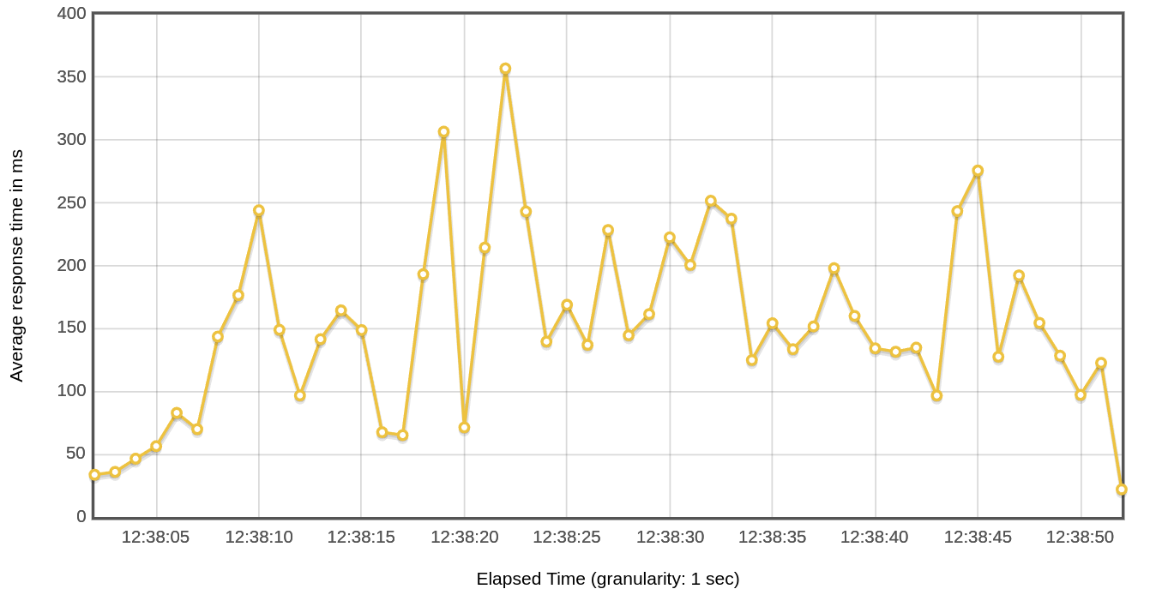
\includegraphics[width=\linewidth]{obrazky-figures/perf/local_metal_30_responseTimesOverTime.png} \\[\abovecaptionskip]
    \small (a) Průběh latence odpovědi od serveru v~čase pro 30 současných uživatelů.
  \end{tabular}

  \vspace{\floatsep}

  \begin{tabular}{@{}c@{}}
    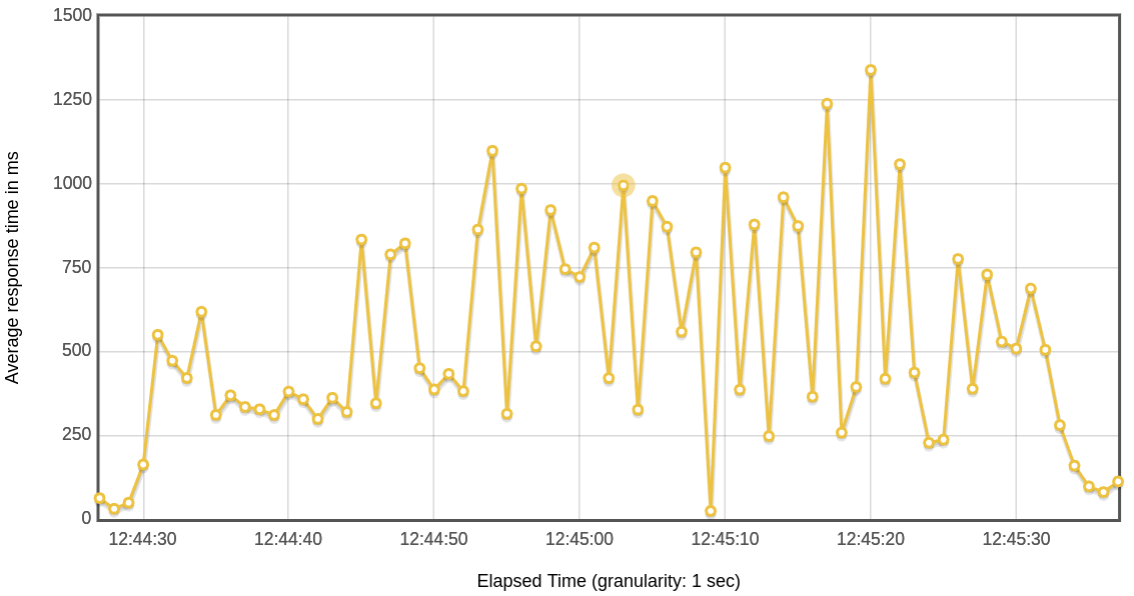
\includegraphics[width=\linewidth]{obrazky-figures/perf/local_metal_100_responseTimesOverTime.png} \\[\abovecaptionskip]
    \small (b) Průběh latence odpovědi od serveru v~čase pro 100 současných uživatelů.
  \end{tabular}

  \caption{Grafy latence serveru při interaktivní simulaci.}
  \label{responseTimes}
\end{figure}

\section{Testování webu}

Webová část projektu byla testována především manuálně.
Uživatelská rozhraní jsou proměnlivá a automatizace jejich testování je časově náročné.
Vývoj probíhal v~prohlížeči Google Chrome.
V~rámci testování byl také proveden manuální test funkcionality v~prohlížeči Mozilla Firefox.
Takto byly pokryty dva nejpopulárnější prohlížeče a tím i software většiny uživatelů.

Testování proběhlo na zařízeních různé výkonnosti a formátu.
Vývojové nástroje poskytují možnost uměle omezit výkon zařízení a rychlost připojení pro zjednodušení testování aplikace v~širokém spektru situací.

Moduly webové aplikace byly v~porovnání se simulátorem testovány mnohem méně.
Testování zde bylo zaměřeno pouze na malé izolované funkce.

Z~výkonnostního hlediska byla aplikace sledována naopak více.
Knihovna React (ale i web obecněji) patří k~méně výkonově optimálním řešením uživatelského rozhraní, proto je nutné více dbát na optimalitu implementace.
Vývojové rozšíření prohlížeče pro React poskytovalo kvalitní zpětnou vazbu, díky které byly odhaleny mnohé výkonnostní problémy (viz sekce \ref{optimRender} o~optimalizaci renderování).

% alignment, čitelnost
% Accessibility Testing - try using a screen reader, automated tools

% Tab order, visual order, showing focused element

Automatizovaný nástroj pro testování přístupnosti rozhraní Google Lighthouse odhalil některé nedostatky, jako například špatné značení tlačítek a odkazů pro asistivní technologie.
Odhalil i jeden případ nedostatečného kontrastu textu vůči jeho podkladu.
Nástroj také navrhoval možná řešení těchto problémů.
%TODO: metriky z Lighthouse (LCP)

Výsledky měření odezvy simulace v~milisekundách jsou pouze orientační.
Byly provedeny na stejném počítači jako výkonnostní testování.
Renderování na začátku simulace (s~malým počtem prvků) trvá asi 60\,ms; s~více zaplněnými buffery trvá okolo 80\,ms.

% route announcer
% eslint-plugin-jsx-a11y

\subsection{Uživatelské testování}

V~pozdní fázi vývoje aplikace proběhlo uživatelské testování.
Test proběhl v~podobě online dotazníku se dvěma úkoly, které měl uživatel v~aplikaci splnit.
Dotazník byl rozeslán studentům a pracovníkům FIT VUT.
Dotazník se ptal na úspěšnost splnění úkolů, na celkový dojem z~aplikace, zpětnou vazbu v~podobě ohodnocení v~rozsahu 0-10 bodů a textu ve volné formě.

Ze všech účastníků průzkumu (9 osob) dokázalo splnit oba úkoly 5 osob.
Úspěšnost splnění úkolu byla kontrolována otázkou, kterou bylo možné správně zodpovědět pouze po úspěšném splnění druhého úkolu.

Průměrné hodnocení výukové hodnoty aplikace přesáhlo 9 bodů na stupnici od 0 do 10, kde 10 je nejlepší možné hodnocení.
Hodnocení přehlednosti rozhraní bylo horší s~průměrem 8,4.

Zpětnou vazbu po zpracování vnímám obecně pozitivně.
Jako nejčastější se projevily tyto problémy:
\begin{itemize}
    \item nejasný způsob zadávání dat pro simulaci,
    \item nejasný způsob pohybu \uv{pohledu} v hlavním okně simulace.
\end{itemize}
% povedlo se taky odhalit bug způsobující pád aplikace

Problém se zadáváním dat pravděpodobně souvisel s~rozdělením definice kódu a definice dat do dvou záložek.
Problém jsem se rozhodl vyřešit poskytnutím průvodce aplikací.
Průvodce po krocích předvede načtení jednoho z~příkladů a definici pole s~hodnotami.
Obrázek \ref{walkthrough} ukazuje jeden z~kroků průvodce.
Relevantní část rozhraní je zvýrazněna a je zobrazen krátký vysvětlující komentář. 

\begin{figure}[hbtp]
\centering
    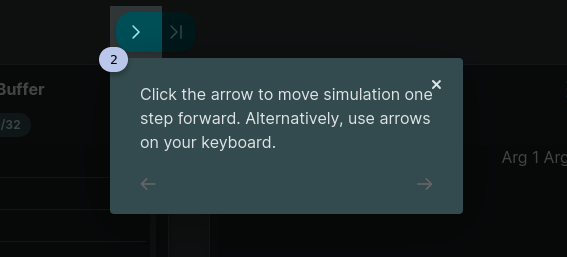
\includegraphics[width=11cm]{obrazky-figures/impl/Walkthrough.png}
    \caption{Průvodce základními funkcemi simulátoru.} 
    \label{walkthrough}
\end{figure}

% TODO Grafy vyhodnocení?

\section{Nasazení}
% build, dependencies

Aplikace je provozována kontejnery technologie Docker.
Docker jsem zvolil z~důvodů konzistence prostředí a jednoduchosti instalace.
První kontejner obsahuje webový server, druhý kontejner obsahuje simulační server.
Oba kontejnery ke komunikaci s~vnějškem otevírají jeden port.
Webový kontejner má síťový přístup do simulačního kontejneru, aby mohl předávat požadavky uživatele.
Součástí repozitáře je skript, který oba kontejnery spustí pomocí \texttt{docker-compose}.

V~případě použití Dockeru je jediným požadavkem instalace Dockeru a internetové připojení.
Jako virtualizační technologie má provoz serveru v~Dockeru nezanedbatelný dopad na výkon, vždy je ale možné aplikaci nainstalovat přímo.

Přímá instalace je detailně dokumentovaná v~textových souborech, které jsou součástí repozitáře a také v příloze \ref{installSteps}.
Je možné se inspirovat i nahlédnutím do kontejnerizačních skriptů, které obsahují přesnou sekvenci příkazů k instalaci a spuštění.
Prerekvizitami jsou programy \emph{Node.js} (runtime pro JavaScript), Java runtime, systém pro automatizaci překladu Gradle a GCC pro RISC-V (\texttt{gcc-riscv-none-elf}).

Knihovní závislosti webové aplikace jsou spravovány systémem NPM\footnote{\url{https://www.npmjs.com/}} (Node Package Manager).
Soubory \texttt{package.json} a \texttt{package-lock.json} specifikují použité knihovny a jejich verze.
Při instalaci jsou závislosti staženy z~centrálního repozitáře.

Proces nasazení je \emph{automatizovaný} službou \emph{GitLab CI/CD}.
Soubor \texttt{.gitlab-ci.yml} v~kořeni projektu definuje předpisy akcí, které se mají spouštět při různých událostech v~repozitáři.
Pro každý commit se spouští testy.
Úspěšnost testů je zobrazena v~grafickém rozhraní GitLabu.
Při novém \emph{Pull Requestu} se spustí server s~aplikací pro otestování a zhodnocení vedoucím.

Konfigurace simulátoru je založena na souboru s~dvojicemi klíč-hodnota.
Existují dvě verze této konfigurace (vývojová a produkční).
Výběr probíhá při startu podle proměnných prostředí.
Parametry lze přepsat argumenty příkazové řádky.
Webová aplikace se konfiguruje proměnnými prostředí.
Jedinou relevantní konfigurací je adresa simulačního serveru.
